\chapter{まとめ}

\section{本論文のまとめ}
HL-LHCに向けてATLAS内部飛跡検出器の総入れ替えを予定しており、これに向けてピクセルモジュールを世界で10,000台生産する予定である。
各モジュールに対して品質試験を行い、全てのモジュール及び品質試験の結果は中央データベースに保存する。

本研究では、この生産及び品質試験に向けてデータベースシステムの構築を行った。
各生産現場にてデータ保存、管理をするローカルデータベースを確立し、品質試験結果検索や中央データベースとの同期機能など、生産時に必要となる諸ツールの開発を行った。

開発した諸ツールを含め、生産において必要な機能の確認を行った。本番を想定したソフトウェア、ハードウェアのセットアップと各ツールの処理実行を達成し、機能が使用可能であることを確認した。

主な開発項目の1つ目として品質試験検索機能を開発し、MongoDB内に新しいコレクションを設ける工夫により、開発当初に問題となった処理時間の改善に成功した。
実際に処理時間の測定を行い、データ数の増加に対しても検索機能が不都合なく使えることを確認した。
本番を想定した見積もりを行い、84,000件のデータ数に対して$2.6\pm0.1$[sec]で処理が実行できる見込みであり、生産時において十分に使える機能であることを確認した。

2つ目に中央データベースとの同期ツールを開発した。
世界的に使われるツールであり、全ての生産現場でこのツールをサポートするために中央データベースへの通信処理時間調査をKEK、LBL、CERNのサーバーを用いて行った。
KEKのサーバーを用いた場合に最も時間がかかることを確認し、このサーバーにおいて十分に使うことができる機能開発を達成すれば世界的に問題がないと考えた。
開発した中央データベース同期ツールについてKEKサーバーを用いて処理速度測定を行った。モジュール情報のダウンロード機能に関して、モジュール1つあたり$4.0\pm 0.4$[sec]の処理時間がかかることを確認した。
生産に向けて処理時間の改善策をいくつか考案し、それぞれについて見積もりを行った。
読み出し試験結果のアップロード機能に関して、処理時間のボトルネックとなっている箇所を分析し、結果ファイルをZIPファイルにまとめ、圧縮しアップロードを行うという改善を加え、処理時間の改善に成功した。
生産時においてモジュール1つに対しての結果アップロード処理時間の見積もりが$1.2\pm 0.1$[min]であり、生産を通して使える機能であることを確認した。

\section{現状と今後の課題}
\subsection{ソフトウェアリリースとユーザサポート}
本論文で述べたツールの他に、読み出し試験コマンド統括ソフト、品質試験結果アップロード用ソフトなどの開発もチームとして行っている。
全てのソフトウェアを含めて、品質試験のデータ管理を達成するようなアプリケーションスイートを目指している。
2020年12月9日にファーストバージョンのリリースを行い、いくつかの機関で全体のシステム及びソフトウェアが使われている現状である。

またCERNで行ったチュートリアルを経て、世界的に機能普及が進んでいる。
そのためユーザサポートとしてソフトウェア使用のためのドキュメント[7-1]の作成、整備も行っている。
開発者の連絡先やローカルデータベース専用掲示板へのリンクもドキュメントに記している。何か問題が生じた時などに簡単に問い合わせができる仕組みを整えている。

\subsection{開発課題}
本研究では検索機能や同期機能など、読み出し試験を対象とした機能を重点的に開発した。
ローカルデータベース開発は、読み出し試験の結果を管理したいという要求から始まり、現在はそれ以外の品質試験も含め、全ての結果や組み立て工程の管理も目標としている。
今後の開発課題として以下の機能をあげる。
\begin{itemize}
  \item 読み出し試験以外(外観検査、平坦性測定等)の結果同期機能.
  \item 中央データベースからローカルデータベースへ品質試験結果の同期.
  \item 品質試験結果解析とモジュール選別機能. 
  \item 組み立て工程管理を世界的にサポート.
\end{itemize}

最後の項目に関して、モジュールの組み立て工程は各機関ごとに異なるため、全ての現場における工程を調査しそれをサポートするシステムを実装する必要がある。
例えば、日本では「ベアモジュール・フレキシブル基板貼り付け」工程の後に、モジュール冷却のための構造である「セル搭載」を行う予定であり、これは他の組み立て機関とは異なる。
各地域における柔軟な生産を許しているため、組み立て工程は世界的に統一されていない。
データベースシステムでは多様な組み立て工程に対応できるシステムとする必要がある。

このシステム実装において、中央データベースには選択可能な組み立て工程を定義する機能が存在し、これを使用することを考えている。
そのイメージを図\ref{optional_stage}に示す。

\begin{figure}[bpt]\centering
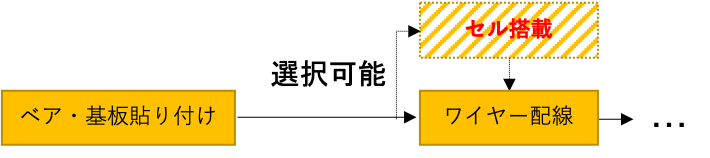
\includegraphics[width=10cm]{optional_stage}
\caption[中央データベースにおける選択可能な組み立て工程のイメージ]{中央データベースにおける選択可能な組み立て工程のイメージ。図に示すように中央データベースでは選択可能な組み立て工程を定義することができる。図ではセル搭載が選択可能となっていて、ベア・基板貼り付け工程の後に、どちらの工程に進むのかを選択できる。この機能を用いて世界的に多様な組み立て工程をサポートすることを考えている。}
\label{optional_stage}
\end{figure}

以下の開発項目をあげる。
\begin{itemize}
  \item 選択式工程の機能を使い、全ての組み立て機関における工程を中央データベース上に定義.
  \item 本研究で開発した同期ツールを拡張、ローカルデータベース上にも中央データベースと同様の組み立て工程構造を保持.
\end{itemize}

これらを達成することにより、全ての機関における組み立て工程情報の管理ができるようになると考えている。


